\documentclass{article}
\usepackage{amsmath}
\usepackage{graphicx}
\usepackage{float}
\usepackage{caption}
\usepackage{subcaption}
\usepackage{blindtext}

\title{Handwriting Recognition using Neural Networks and Image Processing}
\date{5th November 2015}
\author{Akash Rana,
		 Dhruv Reshamwala,
		 Kishore Saldanha,
		 Riyansh Karani}
% \college{DJ Sanghvi College of Engineering}
% \coursename{Final Year Project}
% \coursenumber{1}
% \coursesection{1}
% \instructor{someone}
% \studentnumber{60001120041\ \ \  60001120042\ \ \ \ \ \ \ \ \ \ \ \ \ \ 60001120043\ \ \ \ \ \ \ \ \ \ \ 60001120021}
\begin{document}

	\pagenumbering{gobble}
	\maketitle	
	\newpage
	\pagenumbering{arabic}
	\section{Image Processing}
	\subsection{Convolution}

		\subsubsection{Introduction}
			\paragraph{}
			In mathematics and, in particular, functional analysis, convolution is a mathematical operation on two functions, producing a third function that is typically viewed as a modified version of one of the original functions, giving the area overlap between the two functions as a function of the amount that one of the original functions is translated. For continuous functions $f(x,y)$ and $g(x,y)$, the convolution operation is defined as following :\\ \\ 
			$(f*g)(x,y) = \int\int f(x-u,y-v) g(u,v) du dv$
		
			\paragraph{}
			In the case of discrete signals, the integral takes the form of summation. Hence, in the discrete domain, convolution of two discrete signals $f(x,y)$ and $g(x,y)$ is given as : \\ \\
			$(f*g)(x,y) = \sum_{u}\sum_{v}f(x-u,y-v)g(u,v)$

			\paragraph{}
			Convolution is widely used in Image Processing, as an operation of filtering in the spatial domain. In our case, convolution operations will be performed between a 2D Grayscale image, and a convolution kernel.

		\subsubsection{Steps involved in 2D convolution of an Image with a convolution kernel}
			\begin{enumerate}
				\item Generate a convolution kernel, depending on the application for which convolution is used.
				\item Rotate the mask by $180^{\circ}$ so that the result of convolution does not have to be rotated by $180^{\circ}$.
				\item Apply padding to the image, so that the entire convolution kernel fits inside the image. The number of padding pixels outside the image should be $(size\ of\ convolution\ kernel\ - 1)$.
				\item For every pixel in the image, apply element wise matrix multiplication of the pixel neighborhood of the appropriate size (depending on the size of convolution kernel) and the convolution. Sum all the values of the resultant matrix, and assign the resultant value to the pixel in consideration.\\ \\ \\ \\ \\ \\ \\ \\ 
			\end{enumerate}

			\paragraph{}
			The following is the result of convolution of an image with the
			$3*3\ mean\ filter\  
			\frac{1}{9}
			\left(
			\begin{matrix}
			1 & 1 & 1 \\
			1 & 1 & 1 \\
			1 & 1 & 1 \\
			\end{matrix}
			\right)
			$

			\begin{figure}[ht!]
				% \centering
				\begin{minipage}{.5\textwidth}
					\centering
					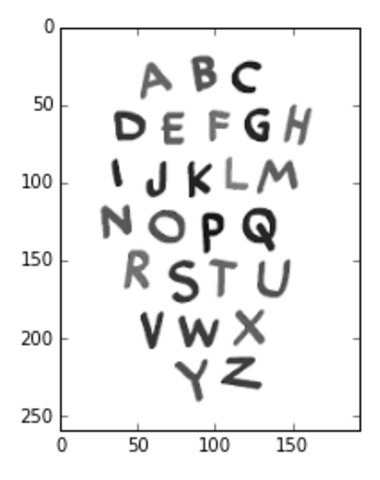
\includegraphics[width=.6\linewidth]{images/original_image.png}
					\captionof{figure}{Before convolution}
					\label{fig:test1}
				\end{minipage}
				\begin{minipage}{.5\textwidth}
					\centering
					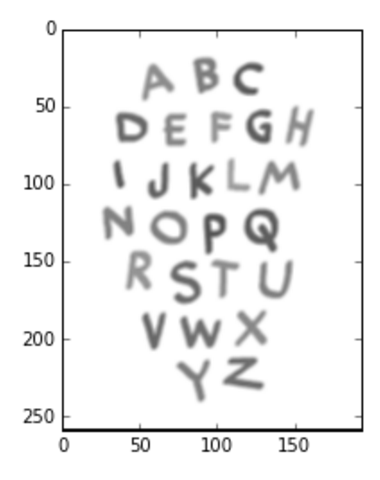
\includegraphics[width=.6\linewidth]{images/mean_filter_after.png}
					\captionof{figure}{After convolution}
					\label{fig:test2}
				\end{minipage}
			\end{figure}

	\subsection{Edge Detection}
		\paragraph{}
		Edge detection is an image processing technique for finding the boundaries of objects within images. It works by detecting discontinuities in brightness. The major importance of edge detection in our project is for the purpose of segmentation of the image into smaller images, for the purpose of object detection.

		\paragraph{}
		There are various methods through which edges can be detected. We have tried various approaches, which have been explained below. 

		\subsubsection{Vertical and Horizontal Edge Detection}
		\paragraph{}
		In this process, two kernels are used to find edges in the vertical and horizontal directions. The corresponding kernels are \\ \\
		$k_{vertical} = 
		\left(
		\begin{matrix}
		1 & 0 & -1 \\
		1 & 0 & -1 \\
		1 & 0 & -1
		\end{matrix}
		\right) 
		and\ \ \ \ 
		k_{horizontal} = 
		\left(
		\begin{matrix}
		 1&   1&   1& \\
		 0&   0&   0& \\
		-1&  -1&  -1&
		\end{matrix}
		\right)
		$

		\paragraph{}
		By convolving the image with the above two kernels separately, we obtain the horizontal and vertical edges as detected in the image.
		\\ \\ \\ \\ \\ 
		\paragraph{}
		The following are the results of applying horizontal and vertical edge detection on an image.
		\begin{figure}[H]
				% \centering
			\begin{minipage}{.5\textwidth}
				\centering
				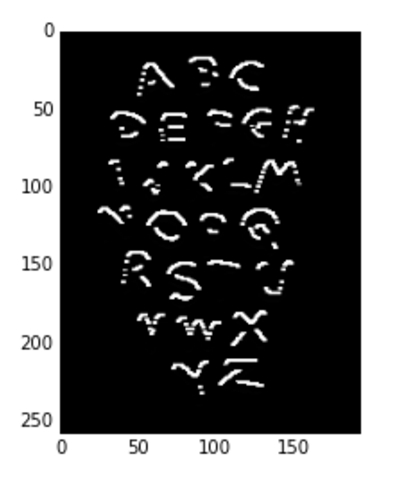
\includegraphics[width=0.6\linewidth]{images/vertical_edge_detection.png}
				\captionof{figure}{After vertical \\ edge detection}
				\label{fig:test4}
			\end{minipage}
			\begin{minipage}{.5\textwidth}
				\centering
				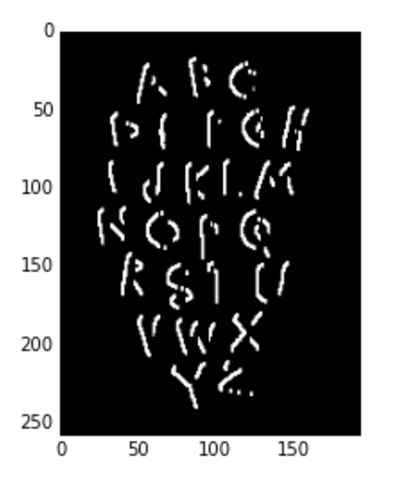
\includegraphics[width=0.6\linewidth]{images/horizontal_edge_detection.png}
				\captionof{figure}{After horizontal \\ edge detection}
				\label{fig:test5}
			\end{minipage}
		\end{figure}

		\paragraph{}
		After this process, the pixel values in the two images can be added to obtain an image that has both horizontal and vertical edges.

		\begin{figure}[H]
			\center
			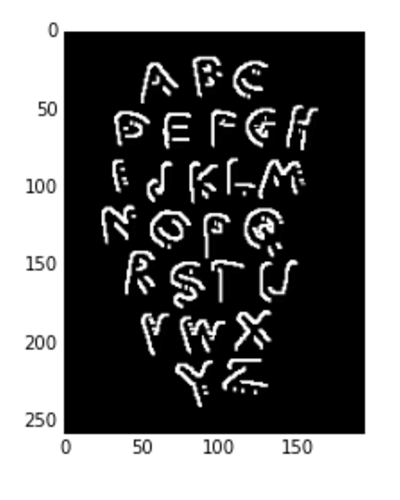
\includegraphics[width=0.3\linewidth]{images/horizontal_and_vertical.png}
			\captionof{figure}{Horizontal plus vertical \\ edge detection}
			\label{fig:text6}
		\end{figure}

		\paragraph{}
		The downside of this approach is that using this method, only one side of the edge can be detected (i.e either black to white or white to black). This problem can be solved using the Full Convolution approach.\\
		\subsubsection{Full Convolution}

		\paragraph{}
		This approach was used to overcome the problems of vertical and horizontal convolution approach. In this approach we calculate four separate convolutions, using four different convolution kernels.

		The first pair of convolutions are done using the convolution kernels that were used in horizontal and vertical convolutions. \\ \\
		$k_{vertical} = 
		\left(
		\begin{matrix}
		1 & 0 & -1 \\
		1 & 0 & -1 \\
		1 & 0 & -1
		\end{matrix}
		\right) 
		and\ \ \ \ 
		k_{horizontal} = 
		\left(
		\begin{matrix}
		 1&   1&   1& \\
		 0&   0&   0& \\
		-1&  -1&  -1&
		\end{matrix}
		\right)
		$

		After the convolution of the image with these two kernels, we convolve the image with two different kernels, shown below : \\ \\
		$k_{vertical} = 
		\left(
		\begin{matrix}
		-1 & 0 & 1 \\
		-1 & 0 & 1 \\
		-1 & 0 & 1
		\end{matrix}
		\right) 
		and\ \ \ \ 
		k_{horizontal} = 
		\left(
		\begin{matrix}
		-1&  -1&  -1& \\
		 0&   0&   0& \\
		 1&   1&   1&
		\end{matrix}
		\right)
		$

		\paragraph{}
		After all the four convolutions are completed, the pixel values of the resultant images from all the four convolutions are summed and the resultant image looks like as shown below : \\


			ASDGASKDLJGALSDKJFLAKSJFLKASDJF\\
			ASDKLJGLAS;DJGL;ASKJDGL;ASDJGL;\\
			KAJSDGLKASJDGLKASDJG;LKADSJG;LA\\
			ASKLDJGLAKSDJGLAKSDJGL;KADJGLKA\\

		\paragraph{}
		As seen in the resultant image, unlike in vertical and horizontal edge detection, all the edges are detected using this method.

		\subsubsection{Sobel-Feldman operator}
		\paragraph{}
		Technically, the Sobel operator is a discrete differentiation operator, computing an approximation of the gradient of the image intensity function. At each point in the image, the result of the Sobel-Feldman operator is either the corresponding gradient vector or the norm of this vector. The Sobel-Feldman operator is based on convolving the image with a small, separable, and integer valued filter in the horizontal and vertical directions and is therefore relatively inexpensive in terms of computations.

		\paragraph{}
		The operator uses two 3×3 kernels which are convolved with the original image to calculate approximations of the derivatives - one for horizontal changes, and one for vertical. If we define A as the source image, and $g_{x}$ and $g_{y}$ are two images which at each point contain the horizontal and vertical derivative approximations, the computations are as follows:

		$g_{x} = 
		\left(
		\begin{matrix}
		-1 & 0 & 1 \\
		-2 & 0 & 2 \\
		-1 & 0 & 1
		\end{matrix}
		\right)
		*A\ \ \ \ \
		and
		\ \ \ \ \ 
		g_{y} = 
		\left(
		\begin{matrix}
		-1&  -2&  -1& \\
		 0&   0&   0& \\
		 1&   2&   1&
		\end{matrix}
		\right)
		*A
		$

		\begin{figure}[H]
				% \centering
			\begin{minipage}{.5\textwidth}
				\centering
				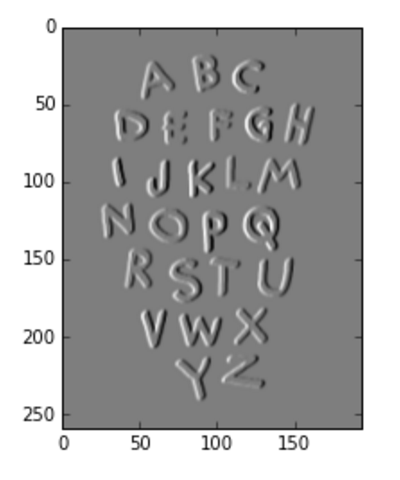
\includegraphics[width=0.6\linewidth]{images/sobel_x.png}
				\captionof{figure}{After convolution with \\ sobel X kernel}
				\label{fig:test6}
			\end{minipage}
			\begin{minipage}{.5\textwidth}
				\centering
				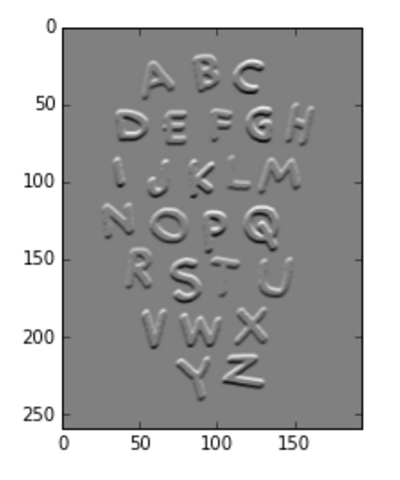
\includegraphics[width=0.6\linewidth]{images/sobel_y.png}
				\captionof{figure}{After convolution with \\ sobel Y kernel}
				\label{fig:test7}
			\end{minipage}
		\end{figure}

		At each point in the image, the resulting gradient approximations can be combined to give the gradient magnitude and the gradient direction, using:\\ \\
		$G = \sqrt{g_{x}^{2} + g_{y}^{2}}$\ \ \ \ \ \ \ \ \ \ \ \ \ \  and \ \ \ \ \ \ \ \ \ \
		$\theta = tan^{-1}(\frac{g_{y}}{g_{x}})$

		\begin{figure}[H]
				% \centering
			\begin{minipage}{.5\textwidth}
				\centering
				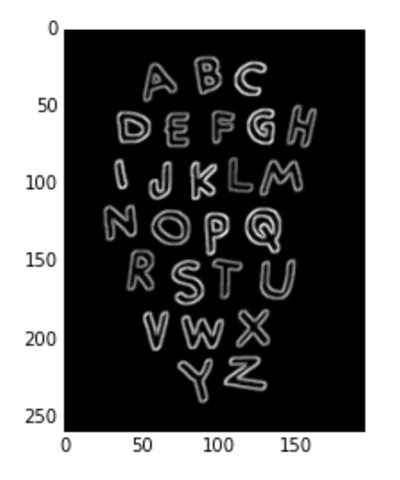
\includegraphics[width=0.6\linewidth]{images/magnitude.png}
				\captionof{figure}{Gradient Magnitude}
				\label{fig:test8}
			\end{minipage}
			\begin{minipage}{.5\textwidth}
				\centering
				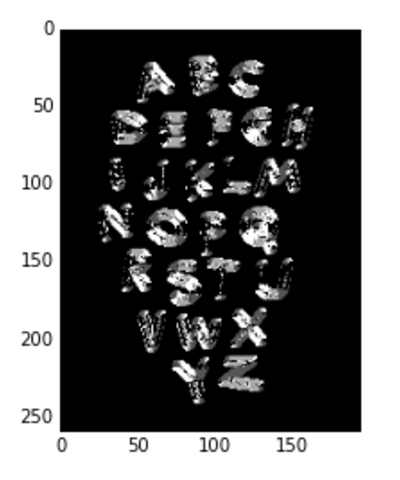
\includegraphics[width=0.6\linewidth]{images/angle.png}
				\captionof{figure}{Gradient Direction}
				\label{fig:test9}
			\end{minipage}
		\end{figure}

		\paragraph{}
		\paragraph{}
		\paragraph{}
		\paragraph{}

		\subsubsection{Laplacian of Gaussian}
		\paragraph{}
		The Laplacian of Gaussian (LoG) filter is another filter, commonly used to detect edges in an image.\\
		\paragraph{Gaussian Filter}
		A Gaussian filter is a filter whose impulse response is a Gaussian function (or an approximation to it). Gaussian filters have the properties of having no overshoot to a step function input while minimizing the rise and fall time. This behavior is closely connected to the fact that the Gaussian filter has the minimum possible group delay. It is considered the ideal time domain filter, just as the sinc is the ideal frequency domain filter. \\
		$G(x) = \frac{1}{2\pi\sigma}e^{\frac{-x^2}{2\sigma^2}}$ \\ \\

		\begin{figure}[H]
			\center
			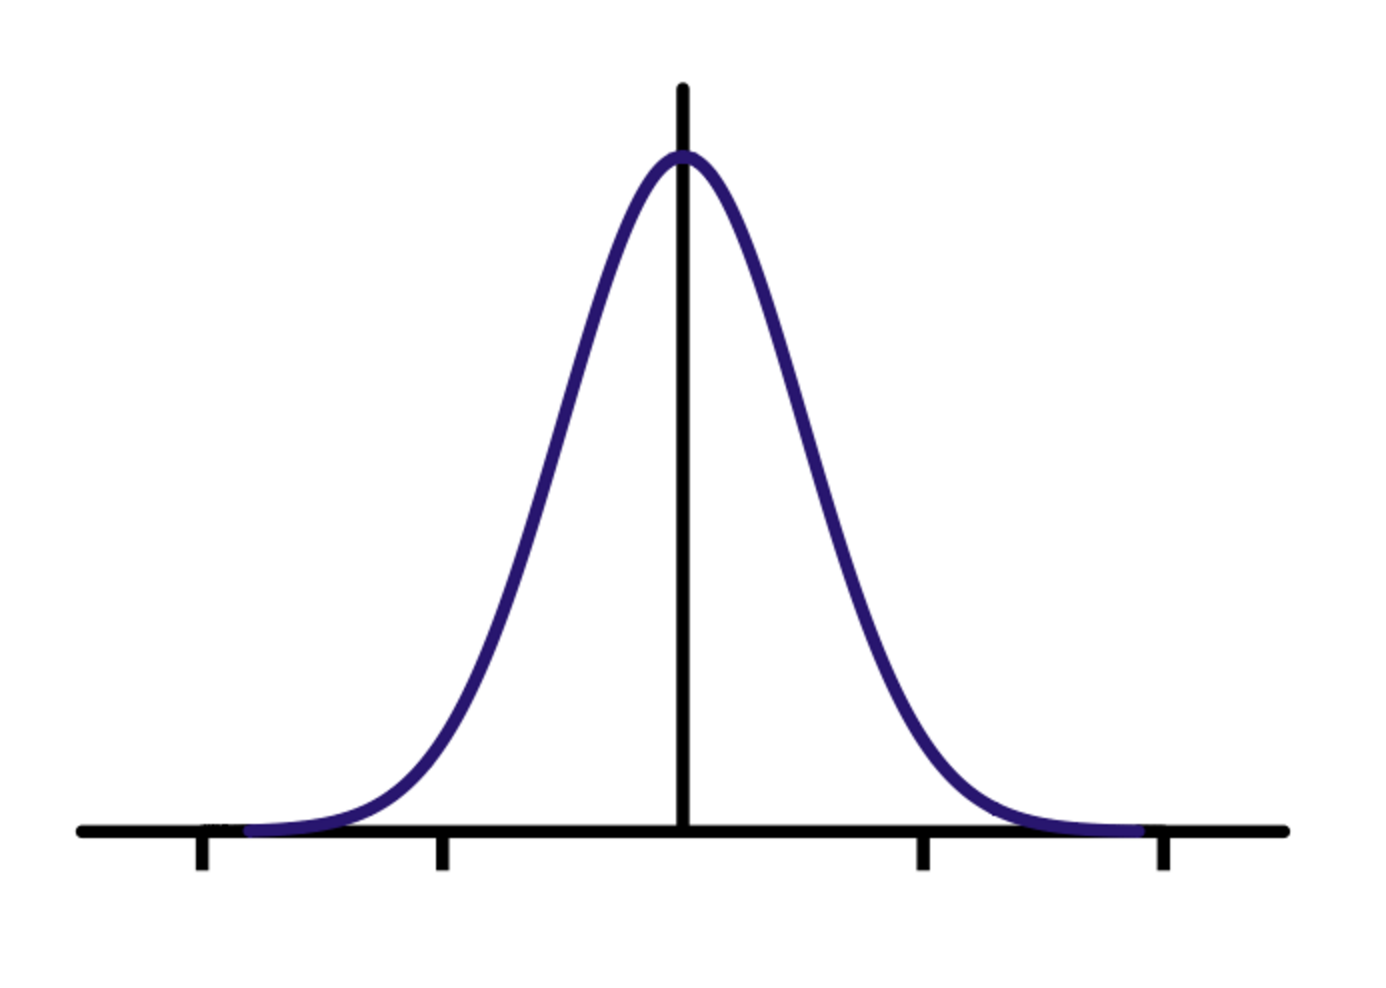
\includegraphics[width=0.3\linewidth]{images/impulse_response_of_gaussian.png}
			\captionof{figure}{Impulse Response of Gaussian Filter}
			\label{fig:text10}
		\end{figure}

		A two variable gaussian filter $(G(x,y))$ can similarly be represented as : \\ 

		$G(x,y) = \frac{1}{2\pi\sigma}e^{\frac{-(x^2 + y^2)}{2\sigma^2}}$ \\ \\		
		\begin{figure}[H]
			\center
			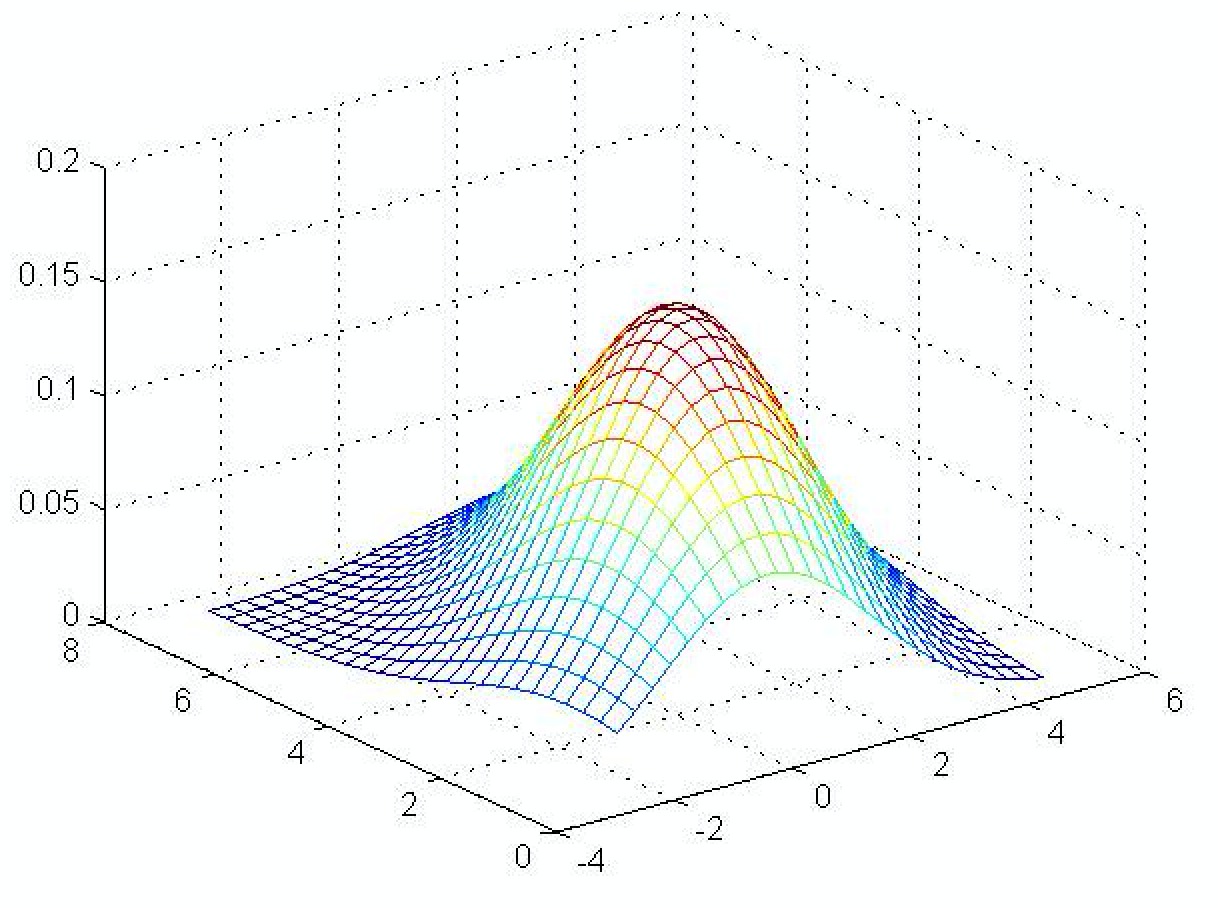
\includegraphics[width=0.3\linewidth]{images/2d_gaussian.png}
			\captionof{figure}{Gaussian Function of \\ two variables}
			\label{fig:test11}
		\end{figure}
		\paragraph{Second Derivative of Gaussian}
		The second derivative of any function is zero, when the function value reaches a maximum or a minimum. Hence, the second derivative of Gaussian filter will provide us with two Zero crossings on either sides of the gaussian peak in the case of Gaussian filter with two variables, and a trough in the case of Gaussian filter with two variables. The second derivative of gaussian is also called the Laplacian of Gaussian.\\ 
		$LoG(x,y) = [\frac{x^2 + y^2 - 2\sigma^2}{\sigma^4}]e^{\frac{-(x^2 + y^2)}{2\sigma^2}}$

		\begin{figure}[H]
				% \centering
			\begin{minipage}{.5\textwidth}
				\centering
				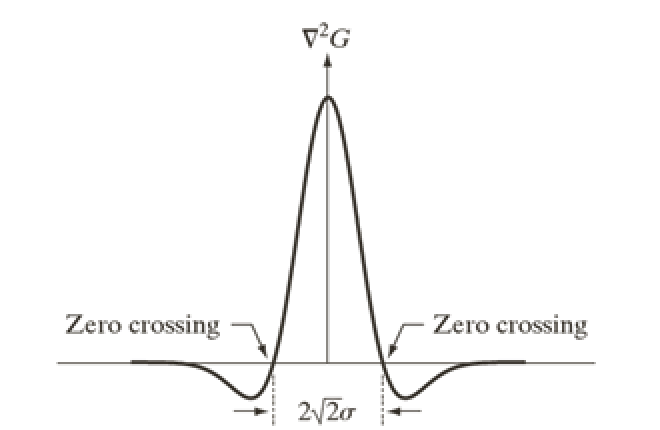
\includegraphics[width=0.6\linewidth]{images/log_1.png}
				\captionof{figure}{Single variable LoG}
				\label{fig:test12}
			\end{minipage}
			\begin{minipage}{.5\textwidth}
				\centering
				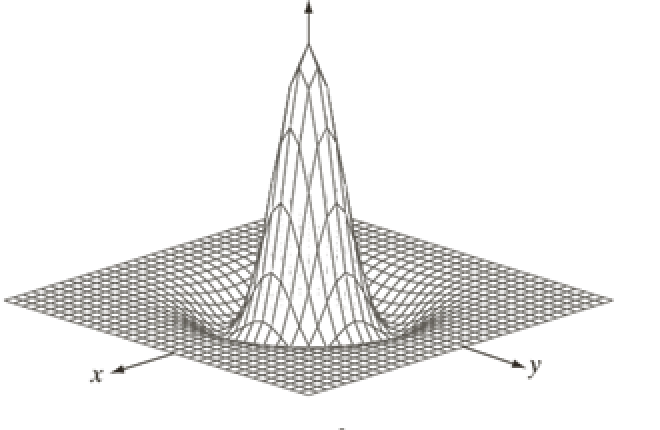
\includegraphics[width=0.6\linewidth]{images/log_2.png}
				\captionof{figure}{Two variable LoG}
				\label{fig:test13}
			\end{minipage}
		\end{figure}

		The following is the result of applying LoG filter to an image and thresholding the LoG image to show edges in the image : 
		
		\begin{figure}[H]
				% \centering
			\begin{minipage}{.5\textwidth}
				\centering
				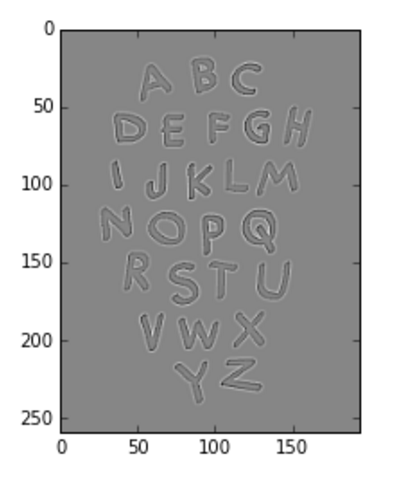
\includegraphics[width=0.6\linewidth]{images/log.png}
				\captionof{figure}{convolution with \\ LoG filter}
				\label{fig:test14}
			\end{minipage}
			\begin{minipage}{.5\textwidth}
				\centering
				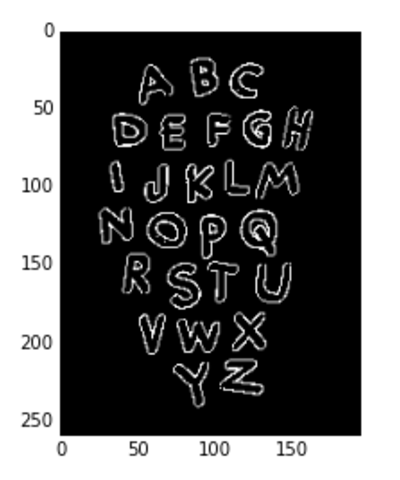
\includegraphics[width=0.6\linewidth]{images/log_threshold.png}
				\captionof{figure}{zero crossings in \\ LoG filtered image}
				\label{fig:test15}
			\end{minipage}
		\end{figure}

	\subsection{Edeg Thinning}
		Edge thinning is a technique used to remove the unwanted spurious points on the edges in an image. This technique is employed after the image has been filtered for noise (using median, Gaussian filter etc.), the edge operator has been applied to detect the edges and after the edges have been smoothed using an appropriate threshold value. This removes all the unwanted points and if applied carefully, results in one pixel thick edge elements.\\
		There are various methods of applying edge thinning, two of which are shown below : \\ \\ \\ \\ \\ \\
		\subsubsection{Non-Maximum supression}
		Non-Maximum suppression is applied to thin the edge. After applying gradient calculation, the edge extracted from the gradient value is still quite blurred. There should only be one accurate response to the edge. Thus non-maximum suppression can help to suppress all the gradient values to 0 except the local maximal, which indicates location with the sharpest change of intensity value. So, basically, non-maximum supression finds the local maximum in the direction perpendicular to the edge.

		\paragraph{}
		The steps involved in implementing the non-maximum supression algorithm are as follows : 
		\begin{enumerate}
			\item Compare the edge strength of the current pixel with the edge strength of the pixel in the positive and negative gradient directions.

			\item If the edge strength of the current pixel is the largest compared to the other pixels in the mask with the same direction(i.e., the pixel that is pointing in the y direction, it will be compared to the pixel above and below it in the vertical axis), the value will be preserved. Otherwise, the value will be suppressed.

		\end{enumerate}
		In some implementations, the algorithm categorizes the continuous gradient directions into a small set of discrete directions, and then moves a 3x3 filter over the output of the previous step (that is, the edge strength and gradient directions). At every pixel, it suppresses the edge strength of the center pixel (by setting its value to 0) if its magnitude is not greater than the magnitude of the two neighbors in the gradient direction. For example,

		\begin{enumerate}
			\item If the rounded gradient angle is $0^{\circ}$ (i.e. the edge is in the north–south direction) the point will be considered to be on the edge if its gradient magnitude is greater than the magnitudes at pixels in the east and west directions.

			\item If the rounded gradient angle is $90^{\circ}$ (i.e. the edge is in the east–west direction) the point will be considered to be on the edge if its gradient magnitude is greater than the magnitudes at pixels in the north and south directions.

			\item If the rounded gradient angle is $135^{\circ}$ (i.e. the edge is in the northeast–southwest direction) the point will be considered to be on the edge if its gradient magnitude is greater than the magnitudes at pixels in the north west and south east directions.

			\item If the rounded gradient angle is $45^{\circ}$ (i.e. the edge is in the north west–south east direction) the point will be considered to be on the edge if its gradient magnitude is greater than the magnitudes at pixels in the north east and south west directions.
		\end{enumerate}

		In more accurate implementations, linear interpolation is used between the two neighbouring pixels that straddle the gradient direction. For example, if the gradient angle is between 45° and 90°, interpolation between gradients at the north and north east pixels will give one interpolated value, and interpolation between the south and south west pixels will give the other (using the conventions of last paragraph). The gradient magnitude at the central pixel must be greater than both of these for it to be marked as an edge.

		The following are the results, when non-maximum supression algorithm is applied to an image : 
		\paragraph{}
		The following are the results of applying erosion operation on an image :
		\begin{figure}[H]
				% \centering
			\begin{minipage}{.5\textwidth}
				\centering
				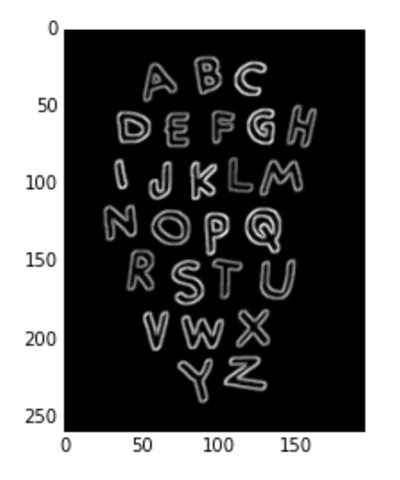
\includegraphics[width=0.6\linewidth]{images/before_non_maximum_supression.png}
				\captionof{figure}{Before Non-Maximum \\ supression}
				\label{fig:test16}
			\end{minipage}
			\begin{minipage}{.5\textwidth}
				\centering
				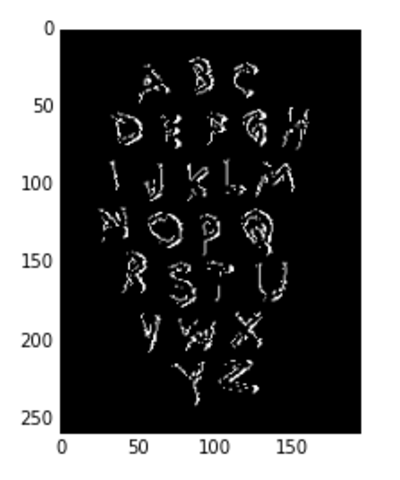
\includegraphics[width=0.6\linewidth]{images/after_non_maximum_supression.png}
				\captionof{figure}{After Non-Maximum \\ supression}
				\label{fig:test17}
			\end{minipage}
		\end{figure}

		\subsubsection{Image Erosion}
		\paragraph{}
		Erosion is one of two fundamental operations in morphological image processing from which all other morphological operations are based. It was originally defined for binary images, later being extended to grayscale images, and subsequently to complete lattices.\\
		The basic idea in binary morphology is to probe an image with a simple, pre-defined shape, drawing conclusions on how this shape fits or misses the shapes in the image. This simple probe is called structuring element, and is itself a binary image.\\
		The erosion of an image $A$ with a structuring element $B$ is defined as the following : \\
		$A\Theta B = \{z|(B)_{z} \subseteq A \}$\ \ \ \ \ \ \ \ \ \ \ \ \ \ \ or \ \ \ \ \ \ \ \ \ \ \ \ \ \ \ $A\Theta B = \{z|(B)_{z}\bigcap A^{c} = \phi \}$

		\paragraph{}
		\paragraph{}
		\paragraph{}
		The following are the results of applying erosion operation on an image :
		\begin{figure}[H]
				% \centering
			\begin{minipage}{.5\textwidth}
				\centering
				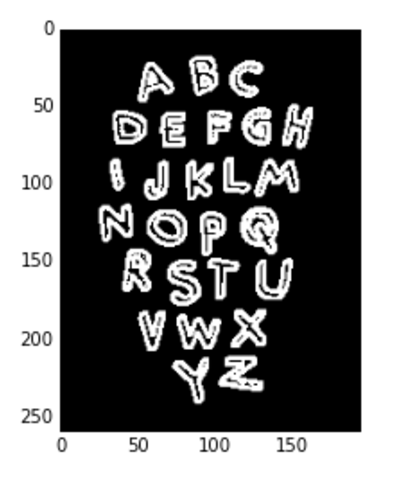
\includegraphics[width=0.6\linewidth]{images/before_erosion.png}
				\captionof{figure}{Before Erosion}
				\label{fig:test18}
			\end{minipage}
			\begin{minipage}{.5\textwidth}
				\centering
				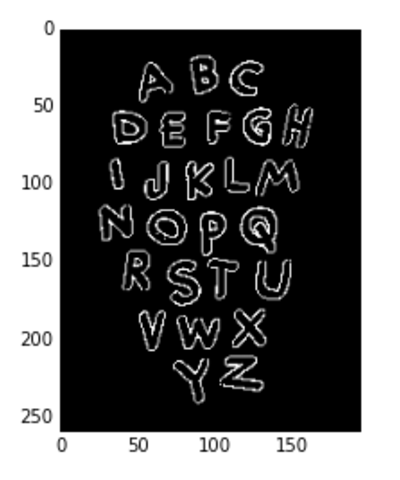
\includegraphics[width=0.6\linewidth]{images/after_erosion.png}
				\captionof{figure}{After erosion}
				\label{fig:test19}
			\end{minipage}
		\end{figure}

	\subsection{Connected Component Labelling}
	Connected-component labeling is an algorithmic application of graph theory, where subsets of connected components are uniquely labeled based on a given heuristic. Two most popular connedted component labelling algorithms are : 

	\paragraph{One component at a time}
	This is a fast and very simple method to implement and understand. It is based on graph traversal methods in graph theory. In short, once the first pixel of a connected component is found, all the connected pixels of that connected component are labelled before going onto the next pixel in the image. In order to do that a linked list is formed that will keep the indexes of the pixels that are connected to each other.

	\paragraph{}
	It is assumed that the input image is a binary image, with pixels being either background or foreground and that the connected components in the foreground pixels are desired. The algorithm steps can be written as:

	\begin{enumerate}
		\item Start from the first pixel in the image. Set curlab (short for 
		current label) to 1.
		\item If this pixel is a foreground pixel and it is not already labelled, then give it the label curlab and add it as the first element in a queue, then go to (3). If it is a background pixel, then repeat (2) for the next pixel in the image.
		\item Pop out an element from the queue, and look at its neighbours (based on any type of connectivity). If a neighbour is a foreground pixel and is not already labelled, give it the curlab label and add it to the queue. Repeat (3) until there are no more elements in the queue.
		\item Go to (2) for the next pixel in the image and increment curlab by 1.

	\end{enumerate}

	\paragraph{Two-pass}
	Relatively simple to implement and understand, the two-pass algorithm iterates through 2-dimensional, binary data. The algorithm makes two passes over the image: the first pass to assign temporary labels and record equivalences and the second pass to replace each temporary label by the smallest label of its equivalence class.

	\paragraph{}
	Connectivity checks are carried out by checking neighbor pixels' labels (neighbor elements whose labels are not assigned yet are ignored), or say, the North-East, the North, the North-West and the West of the current pixel (assuming 8-connectivity). 4-connectivity uses only North and West neighbors of the current pixel. The following conditions are checked to determine the value of the label to be assigned to the current pixel (4-connectivity is assumed)\\

	Conditions to check:
	\begin{enumerate}

		\item Does the pixel to the left (West) have the same value as the current pixel?
		\begin{enumerate}
			\item Yes $-$ We are in the same region. Assign the same label to the current pixel
			\item No $-$ Check next condition
		\end{enumerate}
		
		\item Do both pixels to the North and West of the current pixel have the same value as the current pixel but not the same label?
		\begin{enumerate}
			\item Yes $-$ We know that the North and West pixels belong to the same region and must be merged. Assign the current pixel the minimum of the North and West labels, and record their equivalence relationship
			\item No $-$ Check next condition
		\end{enumerate}

		\item Does the pixel to the left (West) have a different value and the one to the North the same value as the current pixel?
		\begin{enumerate}
			\item Yes $-$ Assign the label of the North pixel to the current pixel
			\item No $-$ Check next condition
		\end{enumerate}

		\item Do the pixel's North and West neighbors have different pixel values than current pixel?
		\begin{enumerate}
			\item Yes $-$ Create a new label id and assign it to the current pixel
		\end{enumerate}

	\end{enumerate}
	The algorithm continues this way, and creates new region labels whenever necessary. Once the initial labeling and equivalence recording is completed, the second pass merely replaces each pixel label with its equivalent disjoint-set representative element.
\end{document}

